%% LyX 1.6.3 created this file.  For more info, see http://www.lyx.org/.
%% Do not edit unless you really know what you are doing.
\documentclass[ngerman]{article}
\usepackage[T1]{fontenc}
\usepackage[latin9]{inputenc}
\usepackage[letterpaper]{geometry}
\geometry{verbose,tmargin=3cm,bmargin=3cm,lmargin=3cm,rmargin=3cm}
\usepackage{babel}

\usepackage{textcomp}
\usepackage{graphicx}
\usepackage[unicode=true, pdfusetitle,
 bookmarks=true,bookmarksnumbered=false,bookmarksopen=false,
 breaklinks=false,pdfborder={0 0 0},backref=false,colorlinks=false]
 {hyperref}

\makeatletter
%%%%%%%%%%%%%%%%%%%%%%%%%%%%%% User specified LaTeX commands.





\usepackage{babel}

%Packages f�r eigen definierte Header und Footer
\usepackage{lastpage}
\usepackage{fancyhdr}
%Nicht einr�cken
%\setlength{\parindent}{0pt}

\def\doctitel{2.Kundengespr�ch} 
\def\docvers{1.0}
\def\docautor{Wolfgang H�ttig, Daniel Br�derle, Michael Schneidt, Ren� Rehn, Firas Zoabi, Tu Xi, Michael Hahn}
\def\docdate{10. Juli 2009}

\makeatother

\begin{document}
%Header und Footer Definitionen f�r das Deckblatt
\thispagestyle{fancy}
\renewcommand{\headrulewidth}{0mm}
\lhead{{\small }}
\chead{{\small }}
\rhead{{\small }}
\lfoot{{\small SIMPL � 2009 \$IMPL}}
\cfoot{{\small \docdate}}
\rfoot{{\small \thepage\ / \pageref{LastPage}}}


%Text f�r das Deckblatt
\vspace*{5cm}
\noindent{\LARGE Studienprojekt SIMPL} \\
\noindent\rule[1ex]{\textwidth}{1pt}
\vspace*{1cm}
\begin{flushleft}
	{\Huge \textbf{\doctitel}} \\
	\vspace{0.5cm}
	{\LARGE Version \docvers} \\
	\vspace{0.5cm}
	{\LARGE \docdate} \\
	\vspace{0.5cm}
	{\LARGE Verfasser: \docautor}
\end{flushleft}
\vspace*{1cm}
\noindent\rule[1ex]{\textwidth}{1pt}

\vspace*{2cm}
\begin{center}
	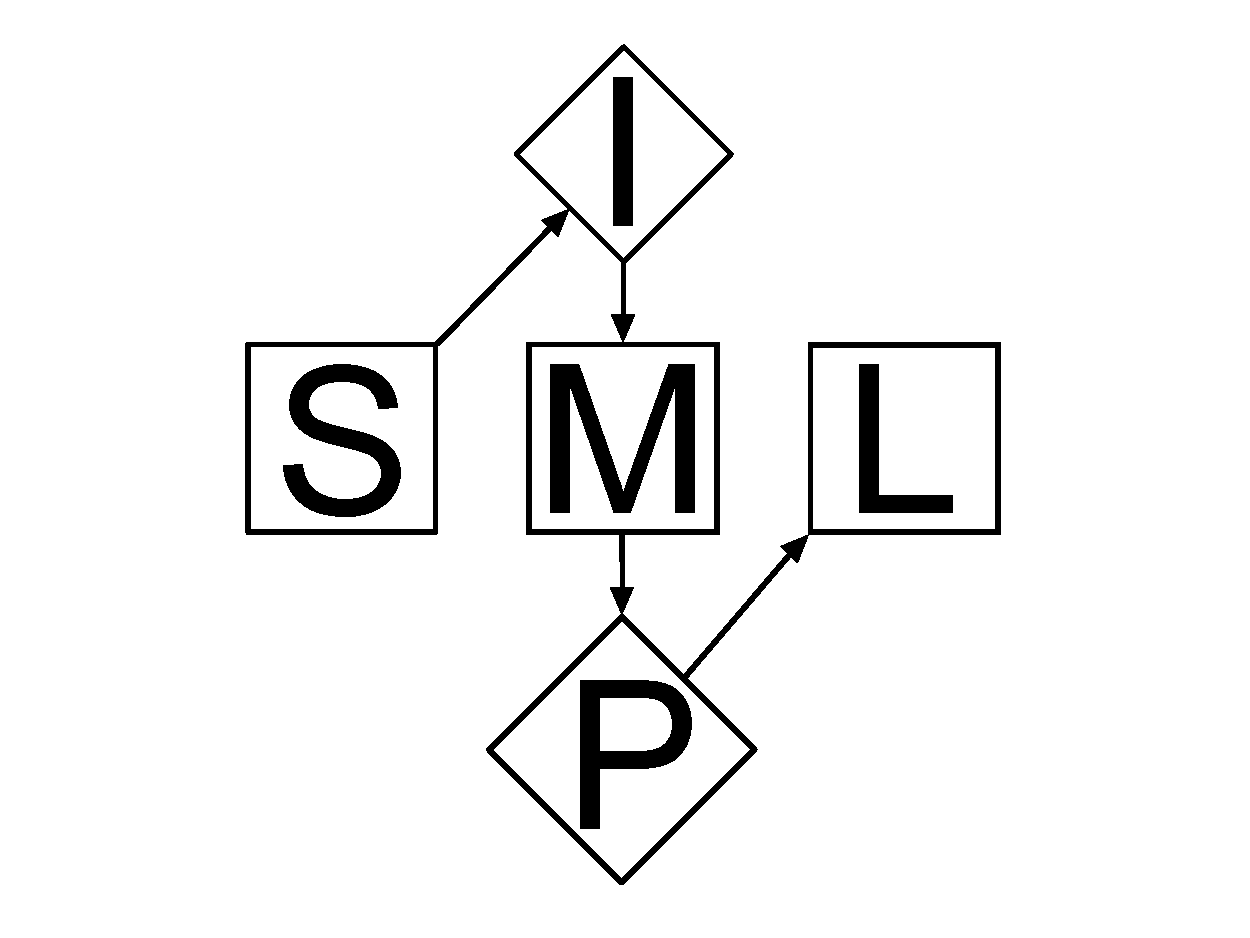
\includegraphics{SIMPL}
\end{center}

%Neue Seite beginnen
\pagebreak{}

%Header und Footer Definitionen f�r alle anderen Seiten
\pagestyle{fancy} \global\long\def\headrulewidth{0mm}
 \lhead{} \chead{} \rhead{} \lfoot{{\small SIMPL � 2009
\$IMPL}} \cfoot{} \rfoot{{\small \thepage\ / \pageref{LastPage}}}

%Ab hier beginnt das Dokument
\tableofcontents{}

\newpage{}


\section{Vertrieb}
\begin{itemize}
\item Folgefrage: F�r welche Datenquellen soll der Zugriff in der Demo gezeigt
werden?

\begin{itemize}
\item A: IBM DB2, OpenSourceDB's: eine RDB und eine XMLDB, evtl. TinyDB
(falls �ffentlich zug�nglich). Ebenso Vorstellung der Monitoring-DB-Anbindung
mit einer der oben genannten.
\end{itemize}
\end{itemize}

\section{Anbindung versch. Datenquellen}
\begin{itemize}
\item Folgefrage: Sollen auch Zugriffe auf mehrere Datenquellen innerhalb
eines Prozess m�glich sein und wie werden diese dann angegeben und
die Queries referenziert?

\begin{itemize}
\item A: Ja, soll m�glich sein. Jede Aktivit�t hat seine eigene Datenquellen-Referenz.
\end{itemize}
\item Folgefrage: Welche Formate werden beim export in lokale Dateien ben�tigt
bzw. sind sinnvoll?

\begin{itemize}
\item A: XML als Standard (siehe IBM Ansatz: RDB-Tabelle <->XML).
\end{itemize}
\item Sollen auch Datenbanken aus einem Prozess heraus erstellt werden k�nnen?

\begin{itemize}
\item A: Nein, Datenbanken existieren bereits. Schema-Definition soll m�glich
sein und das Erstellen, �ndern und L�schen von Tabellen innerhalb
der Schemas.
\end{itemize}
\item Wie wird das Datenbankmanagement realisiert und von wem (Wer setzt
Zugriffsrechte auf der DB)?

\begin{itemize}
\item A: Zugriffsrechte werden in DB gesetzt und sind bereits vorhanden.
\end{itemize}
\end{itemize}

\section{Authentifizierung und Autorisierung der Zugriffe}
\begin{itemize}
\item Wie soll die Angabe von Authentifizierungs- und Authorisierungseinstellungen
�ber den Eclipse BPEL Designer realisisert werden?

\begin{itemize}
\item A: Angaben sollen extra abgefragt und als Nachricht an die DB geschickt
werden.
\end{itemize}
\end{itemize}

\section{Monitoring der Prozessausf�hrung}
\begin{itemize}
\item Muss das vorhandene Monitoring von BPEL und Apache ODE erweitert werden?

\begin{itemize}
\item A: Erweiterung um das Monitoring unserer Funktionalit�ten und die
M�glichkeit eine variable DB als Monitoring-DB anzugeben.
\end{itemize}
\end{itemize}

\section{Sonstige Fragen}
\begin{itemize}
\item Folgefrage: Welche Schritte werden bei der Prozessmodellierung ausgef�hrt,
die die Funktionalit�t des Rahmenwerks nutzen, z.B. 1.Einf�gen einer
SQL-Activity, 2.Datenquelle angeben, 3.Query eingeben, 4.Sicherheitsaspekte
einstellen, ...?

\begin{itemize}
\item A: Test von Queries als Feature (falls zeitlich machbar)
\end{itemize}
\item Folgefrage: Wird das Rahmenwerk direkt in Eclipse als Plug-In ausgef�hrt
oder soll das Rahmenwerk unabh�ngig von Eclipse sein und zus�tzlich
ein Eclipse Plug-In erstellt werden?

\begin{itemize}
\item A: Eclipse Plug-In.
\end{itemize}
\item Auf welcher Infrastruktur l�uft das System sp�ter?

\begin{itemize}
\item A: keine bestimmte, ODE l�uft �berall lokal, DB's verteilt.
\end{itemize}
\end{itemize}

\section{Ist-Analyse}
\begin{itemize}
\item Wie werden im Moment Workflows und BPEL genutzt?

\begin{itemize}
\item A: kein BPEL Einsatz in Scientific Workflows, Realisierung �ber Web-Services.
Kepler, ... definieren eigene Sprachen f�r Scientific Workflows.
\end{itemize}
\end{itemize}

\section{Nichtfunktionale Anforderungen}
\begin{itemize}
\item Wie hoch muss die Skalierbarkeit des Systems sein?

\begin{itemize}
\item A: keine bestimmte Infrastruktur => von schlechten PC's bis zu Supercomputern
alles m�glich
\end{itemize}
\end{itemize}

\section{�nderungsgeschichte}
\begin{itemize}
\item \textbf{Version 0.1}, 06. Juli 2009: Erstellung des Dokuments.
\item \textbf{Version 0.2}, 08. Juli 2009: Erweiterung und �berarbeitung
des Fragenkatalogs.
\item \textbf{Version 1.0}, 10. Juli 2009: Ergebnisse des 2.Kundengespr�chs
wurden eingetragen.
\end{itemize}

\end{document}
